\documentclass[xcolor=table]{beamer}

% Imports:
\usepackage{multirow}
\usepackage{graphicx}
\usepackage{rotating}
%\usepackage{multicol}%for enumerates in several columns
\usepackage[utf8]{inputenc}%
\usepackage{amsmath} %Mathe
\usepackage{amssymb} %Mathe
\usepackage{mathtools}
\usepackage{icomma} % for comma decimals
\usepackage{tikz} % for drawing graphis
\usetikzlibrary{shapes}
\usetikzlibrary{backgrounds}
\usetikzlibrary{positioning}
%\usepackage{esvect}
\usepackage{multicol}%for enumerates in several columns
\usepackage{datetime}
\usepackage{subcaption}
\usepackage[ngerman]{babel}

\usepackage[style=authoryear, backend=biber]{biblatex}
\addbibresource{bibliography.bib}

% Theme of presentation:

\usetheme[]{Frankfurt}%such online
\setbeamertemplate{navigation symbols}{}
\setbeamercolor{section in head/foot}{fg=white, bg=blue!50!black}
\setbeamercolor{title in head/foot}{fg=white, bg=blue!50!black}
\setbeamertemplate{frame numbering}[fraction]
\setbeamercolor{background canvas}{bg=white}
\setbeamercovered{transparent=6}%makes things which are hidden visiable
% Custom settings:
\newcommand{\ew}{\mathbb{E}}
\DeclareMathOperator*{\argmax}{arg\,max}
\usetikzlibrary{arrows}

% First page info:
\title[Belief Propagation]{Preposition Sense Disambiguation}
\subtitle{\textit{TTLab - Text2Scene Praktikum}}
\author{Dirk Neuhäuser
\and 
Tim Rosenkranz
\and 
Tobias Marzell}
\institute[ode]{Prof. Dr. Alexander Mehler, Alexander Henlein}
%\date{\today}
\AtBeginSection[]{
  \begin{frame}
  \vfill
  \centering
  \begin{beamercolorbox}[sep=8pt,center,shadow=true,rounded=true]{title}
    \usebeamerfont{title}\insertsectionhead\par%
  \end{beamercolorbox}
  \vfill
  \end{frame}
}

\makeatletter
\setbeamertemplate{footline}
{
  \leavevmode%
  \hbox{%
  \begin{beamercolorbox}[wd=.333333\paperwidth,ht=2.25ex,dp=2ex,center]{author in head/foot}%
    \usebeamerfont{author in
head/foot}%
  \insertshortauthor\hspace{1em}\beamer@ifempty{\insertshortinstitute}{}{}
  \end{beamercolorbox}%
  \begin{beamercolorbox}[wd=.333333\paperwidth,ht=2.25ex,dp=2ex,center]{title in head/foot}%
    \usebeamerfont{title in head/foot}\insertshorttitle
  \end{beamercolorbox}%
  \begin{beamercolorbox}[wd=.333333\paperwidth,ht=2.25ex,dp=2ex,right]{date in head/foot}%
    \usebeamerfont{date in head/foot}\insertshortdate{}\hspace*{2em}
    \insertframenumber{} / \inserttotalframenumber\hspace*{2ex} 
  \end{beamercolorbox}}%
  \vskip0pt%
}
\makeatother
\begin{document}

\begin{frame}
\titlepage
\end{frame}


\begin{frame}
\tableofcontents
\end{frame}


\section{Aufgabe}
\begin{frame}[t]{Motivation}\vspace{10pt}
Preposition-Sinn wichtig für Verständnis:
\begin{description}
\item \emph{\textbf{Auf} der Wache} bedeutet eigentlich, dass man \textbf{in} dem Gebäude ist
\item \emph{\textbf{Auf} dem Tisch} bedeutet, dass etwas wirklich \textbf{auf} dem Tisch ist
\end{description}
Zur Visualisierung braucht man diese Informationen
\end{frame}


\begin{frame}[t]{Nice to Know}\vspace{10pt}
	SemEval Benchmark:
	\begin{itemize}
		\item \textbf{SemEval-Winner 2007} - Max-Entropy-Ansatz: Accuracy bis 75 \%
		\item \textbf{Litkowski 2013} - Lemmatizer und Dependency-Parser: Accuracy: 86 \%
		\item \textbf{Semi-Supervised(2016)} - Ausnutzen von mehreren Sprachen: Accuracy bis 80 \%
		\item \textbf{Hongyu Gong(2018)} - Geographische Context-Vektoren: Accuracy bis 80 \%
	\end{itemize}
\end{frame}

\begin{frame}[t]{Unsere Aufgabe}\vspace{10pt}
	\begin{itemize}
		\item Datenbeschaffung und -bereinigung 
		\item Trainieren von 2 Taggern (hyperparamter-optimiert)
		\item Einbinden in den Text-Imager
		\item Semi-Supervised Ansatz Wenn möglich einbinden
	\end{itemize}
\end{frame}


\section{Datenbeschaffung und -bereinigung\\(Tim und Dirk)}
\begin{frame}[t]{Daten}
	\begin{itemize}
		\item SemEval 2007 oft als Benchmark Datensatz
		\item schwer zu bekommen online
		\item 34 englische Präpositionen mit insgesamt 224 verschiedene Sinnen
		\item Je preposition 2 xml (Trainingsdata und label-defintionen)
	\end{itemize}
\end{frame}

\begin{frame}[t]{Datenbeispiel}
Trainingsdata:
\begin{figure}
	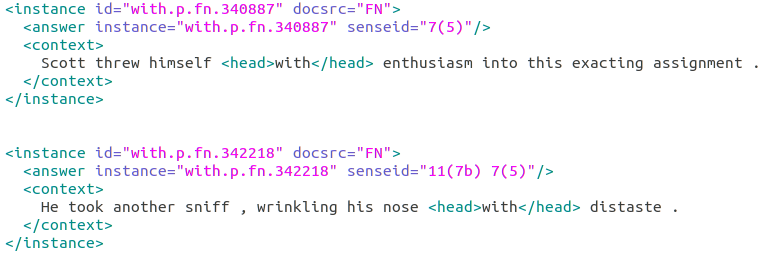
\includegraphics[scale=0.3]{data_example.png}
\end{figure}
Definitionen:
\vspace*{.5cm}
\hspace*{-.8cm}
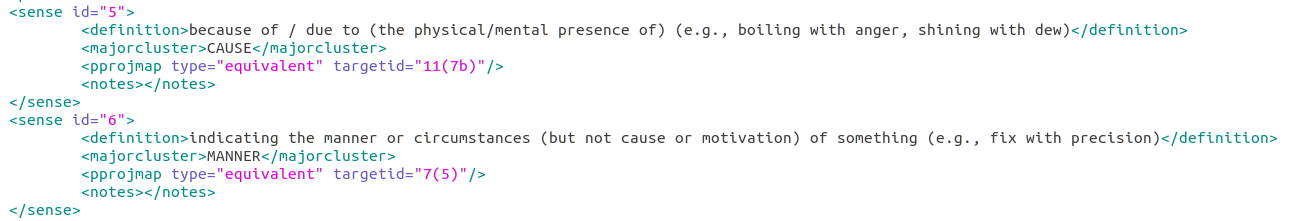
\includegraphics[scale=0.3]{def_example.png}
\end{frame}


\begin{frame}[t]{Aufbereitete Daten}\vspace{40pt}
	\hspace*{-0.75cm}
	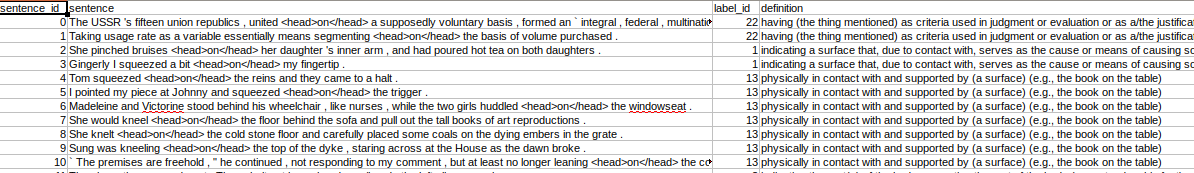
\includegraphics[scale=0.3]{data_cleaned.png}
\end{frame}

\section{Huggingface-Bert\\(Dirk)}
\begin{frame}[t]{Huggingface-Bert}\vspace{10pt}
	Huggingface library:
	\begin{itemize}
		\item Leichte Umsetzung von State-of-the-Art Modellen
		\item Unterstützt bert
	\end{itemize}
	Bert:
	\begin{itemize}
		\item Released: November 2019
		\item Sehr(!) gut vortrainiert
		\item Knackt gleich in mehreren Disziplinen die State-of-the-Art (GLUE, SQuAD, SWAG)
	\end{itemize}
\end{frame}

\begin{frame}[t]{Huggingface-Bert-Trainer}\vspace{10pt}
	\begin{enumerate}
		\item Daten einlesen (90:10 train:val Split)
		\item Daten tokenisieren (pretrained tokenizer von hf für Bert):
			Sätze werden zu \textbf{Input-Ids} und \textbf{Attention-Masks}
		\item bert Modell initialisieren als \textbf{Klassifizierungsmodell} (mit 224 verschiedenen Outputs)
		\item Trainingsschleife
	\end{enumerate}
\end{frame}

\begin{frame}[t]{Huggingface-Bert-Hyperparameter-Optimierung}\vspace{10pt}
	Google empfielt
	\begin{itemize}
		\item Epochen: 4
		\item Optimizer: Adam
		\item Learning-Rate aus [3e-4, 1e-4, 5e-5, 3e-5]
		\item Batch-Size aus [8, 16, 32, 64, 128]
		\item Rest: schon vorgegeben
	\end{itemize}
\end{frame}

\begin{frame}[t]{Huggingface-Bert-Ergebnisse}\vspace{10pt}
	\begin{figure}
		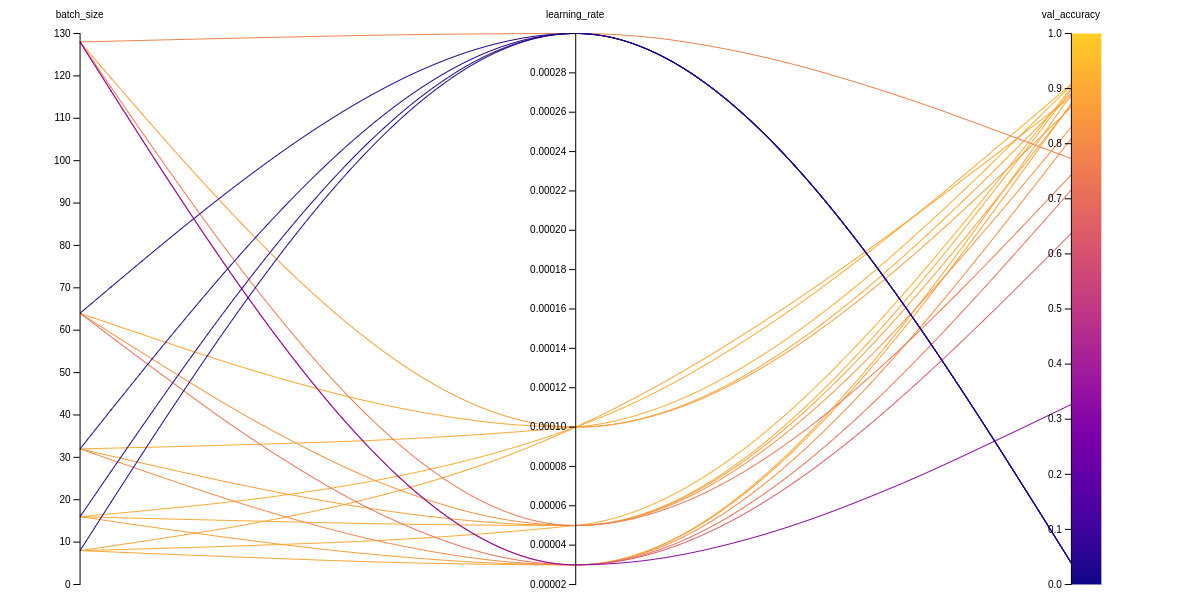
\includegraphics[scale=.25]{hf_overview.png}
	\end{figure}
	Beste Acc: 0.9084 mit Learning-Rate = 1e-4 und Batch-Size = 16
\end{frame}

\begin{frame}[t]{Huggingface-Bert-Ergebnisse}\vspace{10pt}
	\begin{figure}
		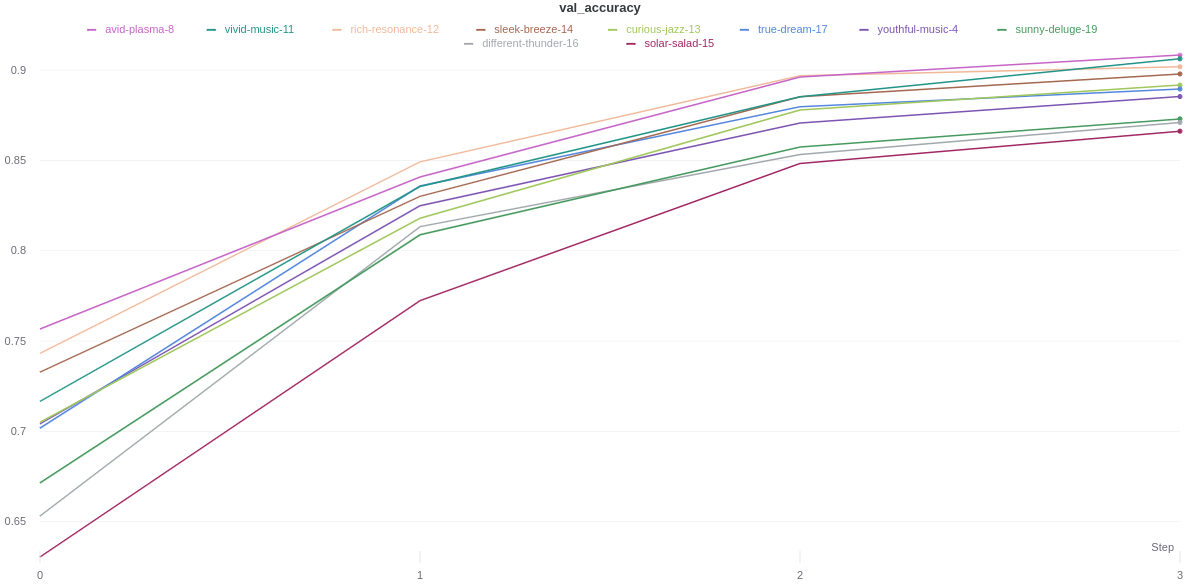
\includegraphics[scale=.25]{hf_acc.png}
	\end{figure}
\end{frame}

\begin{frame}[t]{Huggingface-Bert-Ergebnisse}\vspace{10pt}
	\begin{figure}
		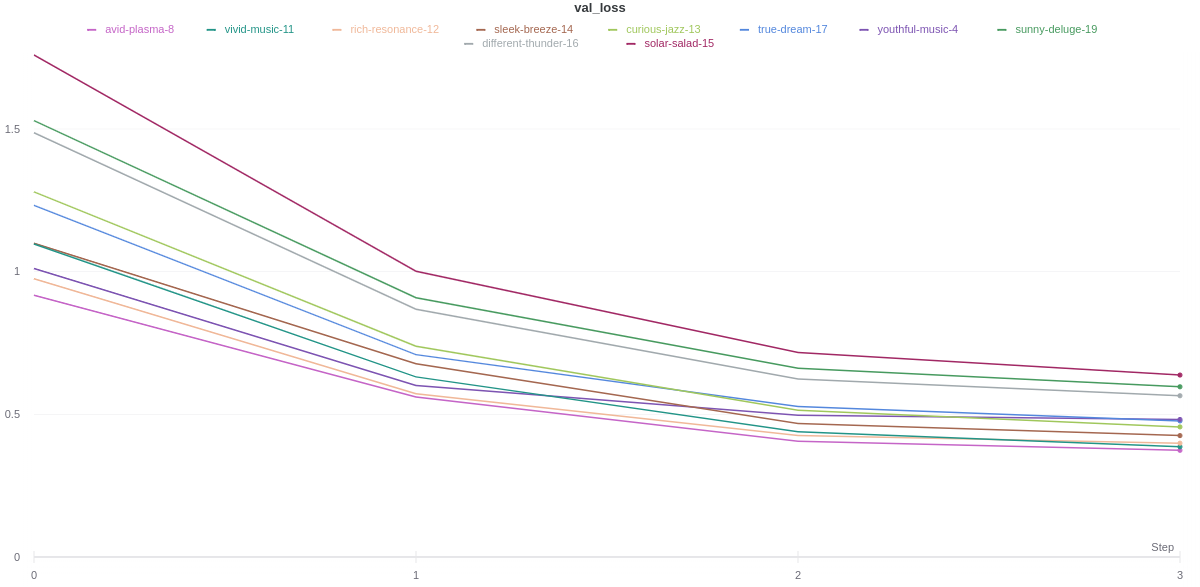
\includegraphics[scale=.25]{hf_loss.png}
	\end{figure}
\end{frame}

\begin{frame}[t]{Huggingface-Bert-Evaluation}\vspace{10pt}
	\only<1>{
		\hspace*{-1cm}
		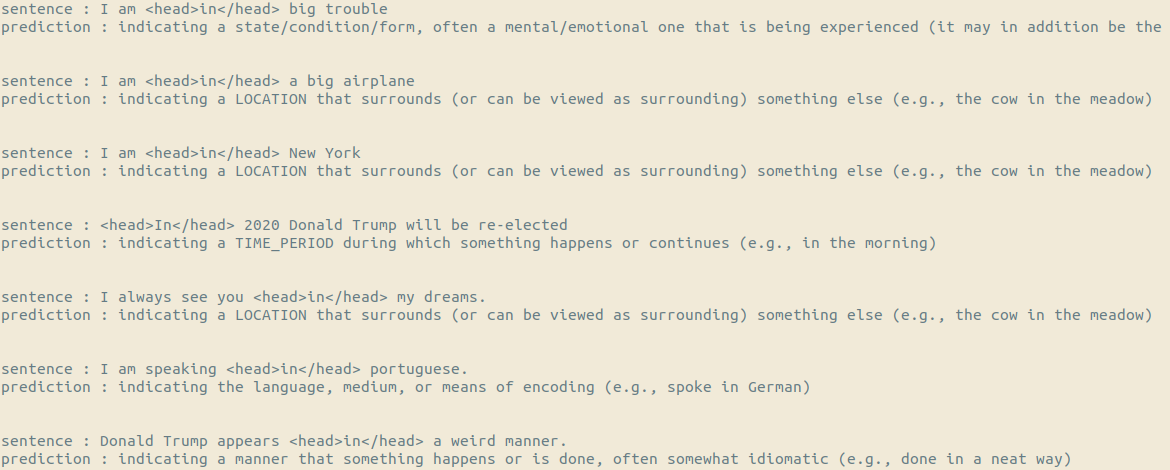
\includegraphics[scale=.4]{in_eval.png}
	}

	\only<2>{
		\hspace*{-1cm}
		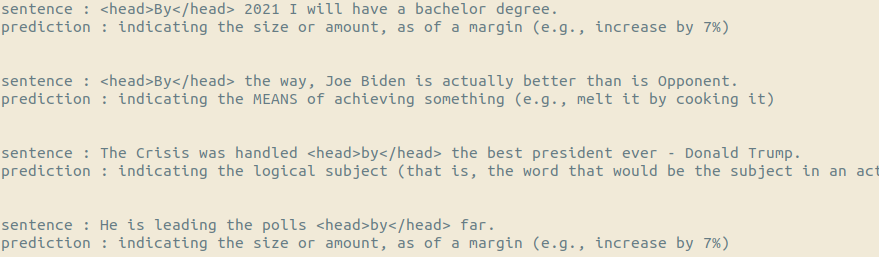
\includegraphics[scale=.4]{by_eval.png}
	}	
\end{frame}

\begin{frame}[t]{Huggingface-Bert-Evaluation-Details}
	\hspace*{3cm}
	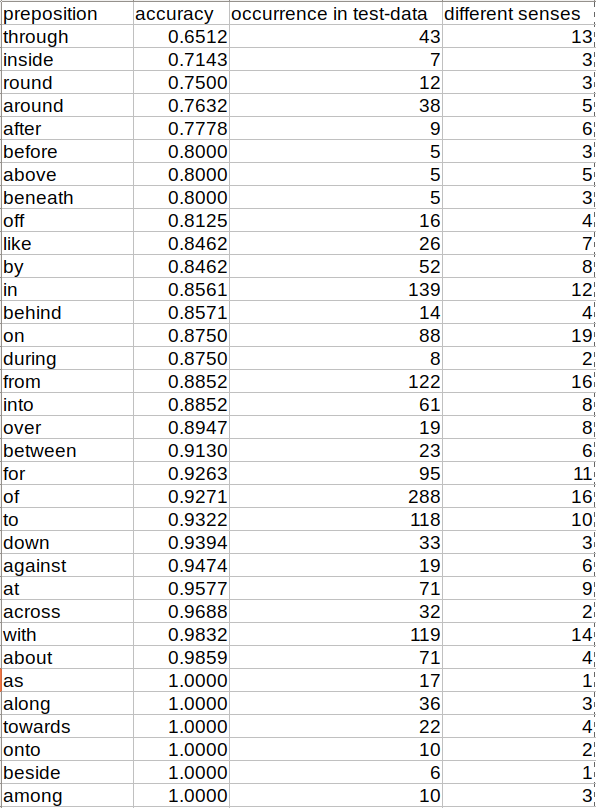
\includegraphics[scale=.25]{hf_details_eval.png}
\end{frame}

\begin{frame}[t]{Huggingface-Bert-Anbindung}\vspace{10pt}
	\hspace*{-1cm}
	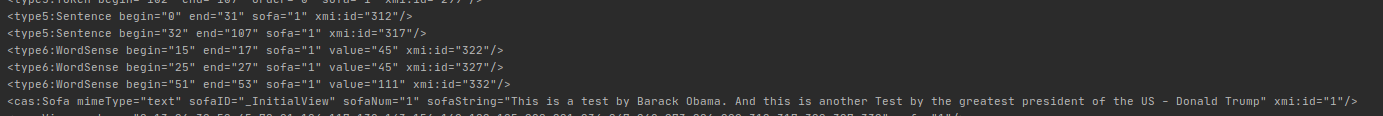
\includegraphics[scale=.25]{einbindung.png}	
\end{frame}


\section{FairNLP\\(Tim)}
\begin{frame}[t]{FlairNLP}\vspace{10pt}
\begin{itemize}
\item Aktuell, spezialisiert für NLP-Aufgaben [\cite{flair}]
\item Einfaches Framework
\item Easy-to-use
\item Basiert auf PyTorch
\end{itemize}
\end{frame}

\begin{frame}[t]{Flair Trainer}\vspace{10pt}
\begin{itemize}
\item Daten im CSV-Format in Korpus laden
\begin{itemize}
\item Mindestens train.csv, optional dev.csv und test.csv
\item dev und test werden ggf. von flair erstellt
\end{itemize}
\end{itemize}
\textbf{Optimisierung:}
\begin{itemize}
\item Optimisierung mit Hyperopt-Wrapper
\item Mehrere Embeddings, Lernraten, etc. eingestellt
\item Unbekannte Fehler
\item log files im repository
\end{itemize}
\end{frame}

\begin{frame}[t]{Flair Optimisierung}\vspace{10pt}
\begin{figure}
	\begin{subfigure}{.4\textwidth}
		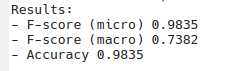
\includegraphics[scale=.3]{flair_results_training1.png}
		
\includegraphics[scale=.3]{flair_acc_opt.png}
		\subcaption*{Ergebnisse des Trainings mit optimierten hyperparameter}
	\end{subfigure}%
	\begin{subfigure}{.3\textwidth}
		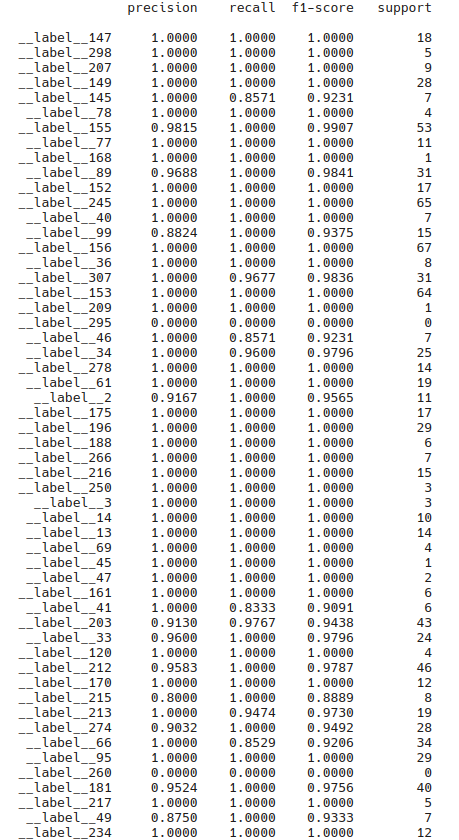
\includegraphics[scale=.25]{flair_results_by_class.png}
		\subcaption*{Ergebnisse je Klasse}
	\end{subfigure}%
	\begin{subfigure}{.3\textwidth}
		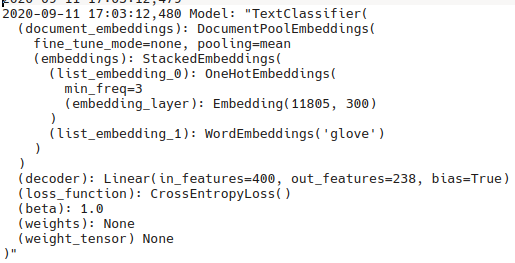
\includegraphics[scale=.3]{flair_best_try.png}
		\subcaption*{Einstellungen der Hyperparameter für gutes Ergebnis}
	\end{subfigure}%
\end{figure}
\end{frame}

\begin{frame}[t]{Flair Ergebnis}\vspace{10pt}
\begin{itemize}
\item Hyperopt-Wrapper nicht gerade zuverlässig
\item FlairEmbeddings anscheinend Problematisch
\item Selbstlernende OneHotEmbeddings mit GloVe-WordEmbeddings = gute accuracy
\item Optimum womöglich noch nicht gefunden
\end{itemize}
\textbf{TextImager}
\begin{itemize}
\item TextImager Einbindung funktioniert problemlos
\item Model in 'resources' Folder legen und/oder Pfad im Code anpassen
\end{itemize}
\end{frame}


\section{Semi-Supervised\\(Tobias)}
\begin{frame}[t]{Datenbeschaffung}\vspace{10pt}
\begin{itemize}
\item European Parliament Proceedings Parallel Corpus 1996-2011 (http://www.statmt.org/europarl/)
\item CDEC Word Aligner (https://github.com/redpony/cdec)
\end{itemize}
\end{frame}

\begin{frame}[t]{Daten Vorbereitung}\vspace{10pt}
\begin{itemize}
\item Tokenizen der Daten
\item Alle Tokens in lower-case überführen
\item Zusammenführen der beiden Corpora (special format)
\item Entfernen von unvollständigen Zeilen
\item Wörter alignen
\end{itemize}
\end{frame}

\begin{frame}[t]{Verfolgte Ansätze}\vspace{10pt}
\begin{itemize}
\item Bidirectional LSTM selbst trainieren
\item Transformers Model transfer learning
\item Bert Transfer Learning
\end{itemize}
\end{frame}

\begin{frame}[t]{Ausblick}\vspace{10pt}
\begin{itemize}
\item Verschiedene Sprachen ausprobieren
\item Output in die anderen Classifier einbinden
\end{itemize}
\end{frame}

\section{Quellen}
\begin{frame}{Quellen}
\printbibliography
\end{frame}

\end{document}
